\section{Discriminant Variables}\label{sec-vh-disc}
The analysis uses a varied set of reconstructed physical variables in the fit to constrain the different processes and control mis-modelling effects. Figure \ref{fig:variablesControlReg} displays the variables used per control regions in the fit, for the resolved regime. Possible variables include the reconstructed mass of the Higgs as $m_{bb}$, $m_{cc}$, or $m_J$, depending on the targeted decay and the regime. The $p_T^V$ is also fitted is some \gls{cr}s, such as the CRHigh in the 2L-channel $TN$ and $BB$ tagged-regions and the $V+l$ \gls{cr} ($LN$-tag). To further boost signal and background seperation in the statistical analysis, dedicated \gls{bdt} are trained with the \textsc{TMVA} Root framework \cite{Therhaag:2011jh} in the combined analysis from dedicated set of event-level input variables to construct a one-dimensional discriminant. \\

\subsection{Multivariate Analysis}
Two sets of discriminants are trained for the analysis: one set of so-called \gls{mva} discrimants for the signal region modelling, and a specific set called mvaCRLow for the CRLow distribution in the resolved $BB$ bin. An additional set of \gls{bdt}s is trained for the cross-check analysis targetting the diboson process as signal, where one of the diboson is $Z$ boson ($WZ$ or $ZZ$) and a $b\bar{b}$ or $c\bar{c}$ pair is expected in the final state. For this, the signal is set to the diboson process decayig into the expected pair of jets ($b\bar{b}$ for $VZ(\rightarrow b\bar{b})$ or $c\bar{c}$ $VZ(\rightarrow c\bar{c})$) and the non diboson processes are set as background.

\begin{figure}[h!]
  %\hspace{-2.0cm}
  \center
  \includegraphics[width=0.98\textwidth]{Images/VH/Discriminants/Variables.pdf}
  \caption{Illustration of the discriminant variables used per control regions of the resolved regime in the fit. Norm-only indicates a region to extract a global normalisation and not binned by a variable.} % Maybe re-do it yourself ...
  \label{fig:variablesControlReg}
\end{figure}

A significant improvement over the boosted \vhb and \vhc analyses in this combined analysis is the wide adoption of \gls{bdt} discriminants in all regimes and targeted Higgs decay, as introduced in the resolved \vhb \cite{ATLAS:2020fcp}. Prior to training, the object and event selections of Section \ref{sec-selectionandcat} and the jet energy corrections of Section \ref{sec-vh-jetcor} are applied. To limit the number of training and the risk of overtraining, the \gls{bdt}s are trained on inclusive regions combining the \gls{sr}s and the $\Delta R$-based \gls{cr}s (CRHigh and CRLow). The \gls{bdt} are trained to discriminate the respective signal of the different targeted decay\footnote{The\vhb samples for \vhb, \vhc samples for \vhc.} from background samples, including $V+$jets, \ttb, single-top, and diboson. \gls{bdt}s were specifically trained in the following categories, differing from the full analysis categorisation to guarantee sufficient statistics and avoid overtraining:

\paragraph{Resolved \boldvhbc:} \gls{bdt}s are trained separately for each tag in the list [$BB$, $TT+TL$, $TN$], with the first targeting \vhb and the latter the \vhc. Seperate trainings were run per lepton channel\footnote{The jet multiplicity only accounts for jets with a $p_T > 30$ GeV.}:
\begin{itemize}
    \item \textbf{0Llepton channel}: separate \gls{bdt}s are trained for the 2-, 3-, and 4-jet categories in an inclusive \ptv $> 150$ GeV region.
    \item \textbf{1L channel}: separate \gls{bdt}s are trained for the 2- and 3-jet categories in two \ptv\ bins: \ptv $\in [75, 150]$ GeV and \ptv $> 150$ GeV.
    \item \textbf{2L channel}: separate \gls{bdt}s are trained for the 2- and 3p-jet categories in two \ptv\ bins: \ptv $\in [75, 150]$ GeV and \ptv $> 150$ GeV.
\end{itemize}
\paragraph{Boosted \vhb:} one \gls{bdt} is trained per lepton channel in an inclusive bin of \ptv $>$ 400 GeV.

For training, the full \gls{mc} statistics is used with GNN truth tagging in all analysis regimes: truth tagging to $BB$ for \vhb, and to $TT$, $TL$, and $TN$ in \vhc. The variables used for each lepton channel in two regimes are listed in Table \ref{tbl:MVAVars}. Variables with long tails are clipped to contain 99\% of the centred distributions and given a specifically chosen default value when they are not defined for an event. More precise definitions of the variables can be found in Appendix \ref{ap-MVA}. The set of features used was subject to a hyperparameter optimisation campaign, with many other variables tested but eventually not included due to their negligible impact on the performance. 

\begin{table}[!htbp]
    \hspace{-1cm}
    %\renewcommand*{\arraystretch}{1.3}
    \newcommand\textunderset[2]{\ensuremath{\underset{\textrm{#1}}{\textrm{#2}}}}
      %\setlength\aboverulesep{0pt}
      %\setlength\belowrulesep{0pt}
      % resize a bit the table 
      %\resizebox{1\textwidth}{!}{ %
      \begin{tabular}{c|ccc|ccc|M{7cm}}
        %\multicolumn{1}{c}{} & \multicolumn{3}{c}{\textunderset{Resolved}{\vhbc}} & \multicolumn{3}{c}{\textunderset{Boosted}{\vhb}} & \multicolumn{1}{c}{}
        \multicolumn{1}{c}{} & \multicolumn{3}{c|}{\vhbc} & \multicolumn{3}{c}{\vhb} & \multicolumn{1}{c}{}\\
        \multicolumn{1}{c}{} & \multicolumn{3}{c|}{Resolved} & \multicolumn{3}{c}{Boosted} & \multicolumn{1}{c}{}
        \\ \hline \hline
        Variable & 0L & 1L & 2L & 0L & 1L & 2L 
        \\ \hline
        $m_{j_1j_2}$ or $m_J$
            & \checkmark & \checkmark & \checkmark 
            & \checkmark & \checkmark  & \checkmark 
            & Mass of Higgs candidate
        \\ \hline
        $m_{{j_1 j_2 j_3}}$ 
            & \checkmark & \checkmark & \checkmark 
            & & &
            & Mass of Higgs candidates and leading additional jet
        \\ \hline
        $p_T^{j_1}$
            & \checkmark & \checkmark & \checkmark 
            & \checkmark & \checkmark & \checkmark 
            & Leading Higgs candidate $p_T$
        \\ \hline
        $p_T^{j_2}$
            & \checkmark & \checkmark & \checkmark 
            & \checkmark & \checkmark & \checkmark 
            & Sub-leading Higgs candidate $p_T$
        \\ \hline
        $p_T^{j_3}$ 
            & & & 
            & \checkmark & \checkmark & \checkmark 
            & Leading non-Higgs candidate $p_T$
        \\ \hline
        $\sum\limits_{i\neq 1, 2}p_T^{j_i}$ 
            & \checkmark & \checkmark & \checkmark 
            & & & 
            & Sum of non-Higgs jet $p_T$
        \\ \hline
        $\Delta R(\textbf{$j_1$}, \textbf{$j_2$}) $
            & \checkmark & \checkmark & \checkmark 
            & \checkmark & \checkmark & \checkmark 
            & Angular separation of Higgs candidates
        \\ \hline
        $\mathrm{bin}_{\mathrm{DL1r}}(j_1)$ 
            & \checkmark & \checkmark & \checkmark
            & \checkmark & \checkmark & \checkmark 
            & Tag bin of $j_1$
        \\ \hline
        $\mathrm{bin}_{\mathrm{DL1r}}(j_2)$ 
            & \checkmark & \checkmark & \checkmark
            & \checkmark & \checkmark & \checkmark 
            & Tag bin of $j_2$
        \\ \hline
        \ptv 
            & $\equiv E_T^{\textrm{miss}}$ & \checkmark  & \checkmark
            & $\equiv E_T^{\textrm{miss}}$ & \checkmark  & \checkmark
            & Vector boson $p_T$
        \\ \hline
        $E_T^{\textrm{miss}}$
            & \checkmark & \checkmark & 
            & \checkmark & \checkmark & 
            & Missing transverse energy
        \\ \hline
        $E_T^{\textrm{miss}}/\sqrt{S_T}$
            & & & \checkmark 
            & & & 
            & Ratio of \etm to sum of jets $p_T$
        \\ \hline
        $|\Delta y(\textbf{$V$},\textbf{$H$})|$
            & & \checkmark & \checkmark
            & & \checkmark & \checkmark
            & Rapidity difference between $V$ and $H$
        \\ \hline
        $|\Delta \phi(\textbf{$V$},\textbf{$H$})|$
            & \checkmark & \checkmark & \checkmark
            & \checkmark & \checkmark & \checkmark
            & Azimuthal angle between $V$ and $H$
        \\ \hline
        $|\Delta \eta(\textbf{$j_1$},\textbf{$j_2$})|$
            & \checkmark & & 
            & & & 
            & Pseudorapidity distance between Higgs candidates
        \\ \hline
        $\min\Delta R(j_i, j)_{i=1,2}$
            & \checkmark & \checkmark & 
            & & & 
            & Smallest angular distance between a Higgs and non-Higgs candidates
        \\ \hline
        $\mathrm{min}[\Delta\phi(\textbf{$l$},\textbf{$j_1$} \textrm{~or~} \textbf{$j_2$})]$
            & & \checkmark  &
            & & & 
            & Smallest $\phi$ between the lepton and a Higgs candidate
        \\ \hline
        $m_{\textrm{eff}}$
            & \checkmark & & 
            & & &
            & Scalar sum of $p_T$ of all small-$R$ jet and \etm
        \\ \hline
        $m_T^W$
            & & \checkmark &
            & & &
            & Transverse mass of the $W$
        \\ \hline
        $m_{\textrm{top}}$
            & & \checkmark &
            & & &
            & Mass of reconstructed leptonically decaying top-quark
        \\ \hline
        $m_{ll}$
            & & & \checkmark 
            & & & 
            & Mass of di-lepton system
        \\ \hline
        $\cos{\theta(\textbf{$l^-$},\textbf{$Z$})}$
            & & & \checkmark 
            & & & \checkmark 
            & $Z$ boson polarisation sensitive angle
        \\ \hline
        $(p_T^{l_1} - E_T^{\textrm{miss}})/p_T^W$
            & & &
            & & \checkmark & 
        \\ \hline
        $p_T^{l}$
            & & &
            & & \checkmark & 
            & \pt imabalance of the lepton and neutrino from $W$ 
        \\ \hline
        $N(\textrm{track-jets in }J)$
            & & & 
            & \checkmark & \checkmark & \checkmark
            & Number of track-jets associated to leading-$R$ jet
        \\ \hline
        $N(\textrm{add. small R-jets})$
            & & & 
            & \checkmark & \checkmark & \checkmark
            & Number of additional small-$R$ jets not matched
        \\ \hline
        Colour
            & & & 
            & \checkmark & \checkmark & \checkmark
            & Variable modelling colour-flow from \gls{qcd}
        \\ \hline \hline
      \end{tabular}
      %}
      \caption{%
        The variables used for the 0-, 1- and 2L channels MVA's in the resolved and boosted regimes for the \vhbc combined analysis. The variables are further described in Appendix \ref{ap-MVA}.}%
      \label{tbl:MVAVars}
    \end{table}
  

The architecture was optimised, with the gradient boosting technique of Section \ref{sec-gradient-boost} used in the resolved regime to improve performance and to capture effects outside the bulk of the distributions. In the boosted regime, due to the lower statistics available and large tails in the distribution, the AdaBoost method - introduced in Section \ref{sub-adaboosted} - is deployed to stabilise training \cite{Adaboost}. Tables \ref{tbl:MVAHyperparams} and \ref{tbl:MVAHyperparams-VHcc} list the architectures used for the \vhb and \vhc \gls{bdt}s respectively, with the main and diboson \gls{bdt}s sharing the same hyperparameters. For \vhc, the hyperparameters are further tuned to avoid overtraining due the limited statistics available in the 2L channel and the diboson cross-check.

\begin{table}[!htbp]
  \renewcommand*{\arraystretch}{1.3}
  \newcommand\textunderset[2]{\ensuremath{\underset{\text{#1}}{\text{#2}}}}
  \centering
    % resize a bit the table 
    \resizebox{1\textwidth}{!}{%
    \begin{tabular}{c|ccc|ccc}
      \multicolumn{1}{c}{} & \multicolumn{3}{c|}{Resolved \vhb} &  \multicolumn{3}{c}{Boosted \vhb} 
      \\\hline \hline
      \textbf{Settings} & 0L & 1L & 2L & 0L & 1L & 2L
      \\\hline
      Boost type 
        & Gradient boost & Gradient boost & Gradient boost % VHbb Resolved 
        & Adaboost       & Adaboost       & Adaboost       % VHbb Boosted 
      \\\hline 
      Number of trees 
        & 200 & 600 & 200 % VHbb Resolved 
        & 800 & 800 & 400 % VHbb Boosted 
      \\\hline 
      Maximum depth
        & 3 & 4 & 4 % VHbb Resolved 
        & 3 & 3 & 3 % VHbb Boosted 
      \\\hline 
      Learning rate ($\beta$) 
        & 0.5 & 0.5 & 0.5% VHbb Resolved 
        & 0.5 & 0.35 & 0.3 % VHbb Boosted 
      \\\hline 
      Number of cuts
        & 100 & 100 & 100% VHbb Resolved 
        & 60  & 60  & 100 % VHbb Boosted 
      \\\hline 
      Minimum node size 
        & 5\% & 5\% & 5\% % VHbb Resolved 
        & 2\% & 2\% & 7\% % VHbb Boosted 
      \\ \hline \hline
    \end{tabular}}%
  \caption{%
    Hyperparameters of the BDTs in the 0L, 1L and 2L channels for the \vhb resolved and boosted. All models used the Gini index as separation method, without pruning.}%
  \label{tbl:MVAHyperparams}
\end{table}


% VHcc use different hyper parameters
\begin{table}[!htbp]
  \renewcommand*{\arraystretch}{1.3}
  \newcommand\textunderset[2]{\ensuremath{\underset{\text{#1}}{\text{#2}}}}
  \centering
    % resize a bit the table 
    %\resizebox{1\textwidth}{!}{%
    \begin{tabular}{c|cc|c}
      \multicolumn{1}{c}{} & \multicolumn{2}{c|}{\vhc} &  $VZ{\rightarrow c\bar{c}}$ signal
      \\\hline \hline
      \textbf{Settings} & 0L, 1L and most 2L regions & 2  3p-jet, low pTV & 0L, 1L and 2L
      \\\hline
      Boost type 
        & Gradient boost & Adaboost % VHcc
        & Adaboost                  % VZcc
      \\\hline 
      Number of trees 
        & 600 & 200 % VHcc
        & 200       % VZcc 
      \\\hline 
      Maximum depth
        & 4 & 4     % VHcc
        & 4         % VZcc
      \\\hline 
      Learning rate ($\beta$) 
        & 0.5 & 0.15 % VHcc
        & 0.15       % VZcc 
      \\\hline 
      Number of cuts
        & 100 & 100  % VHcc
        & 100        % VZcc
      \\\hline 
      Minimum node size 
        & 5\% & 5\%  % VHcc
        & 5\%        % VZcc
      \\ \hline \hline
    \end{tabular}
  %}
  \caption{%
    Hyperparameters of the BDTs in the 0L, 1L and 2L channels of \vhc. The 2L low pTV region mentioned is 75 GeV $<$ pTV $<$ 150 GeV. All models used the Gini index as separation method, without pruning.}%
  \label{tbl:MVAHyperparams-VHcc}
\end{table}


\begin{figure}[h!]
    \hspace{-0.3cm}
    \begin{subfigure}[b]{0.49\textwidth}
        \centering
      \includegraphics[width=\textwidth]{Images/VH/Discriminants/OvertrainCheck_BDT_0L_2J_150ptv_1of2_Test_Output_0L_2jet.pdf}
    \caption{\vhb $BB$-tag model, test AUC = 0.9.} 
    \end{subfigure}
    \begin{subfigure}[b]{0.49\textwidth}
        \centering
      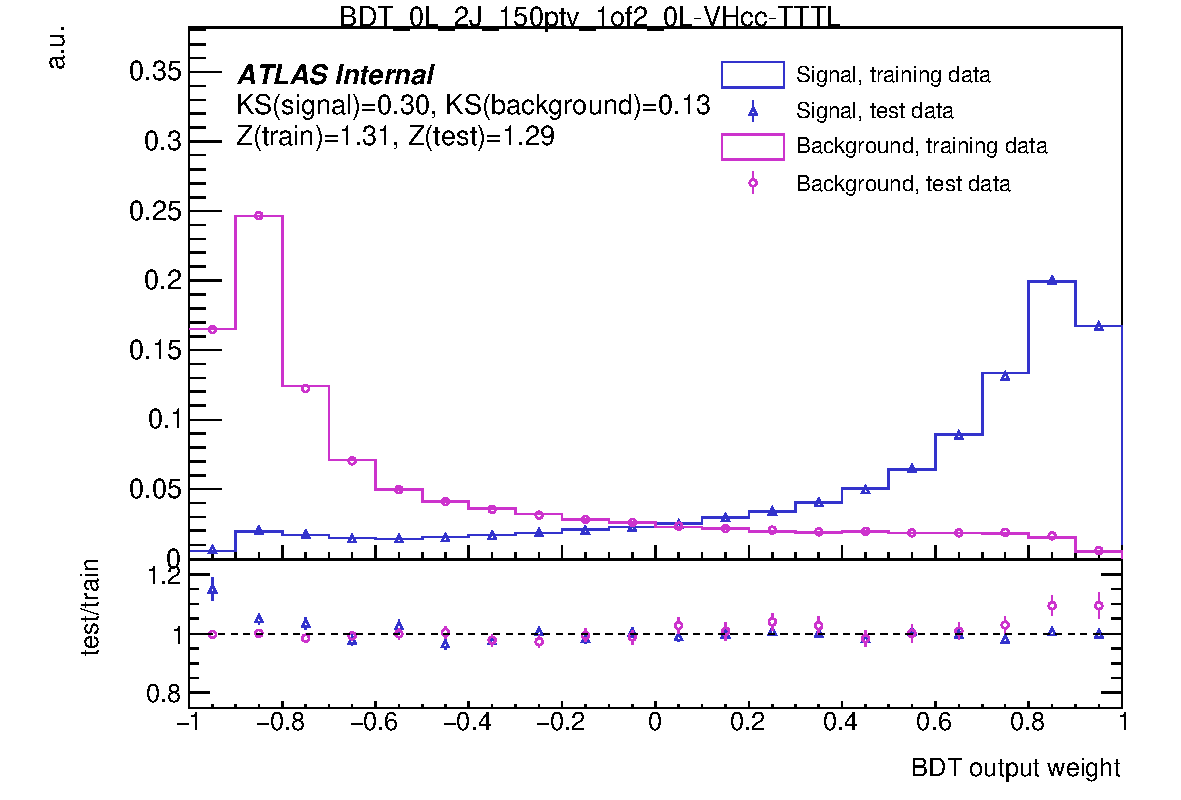
\includegraphics[width=\textwidth]{Images/VH/Discriminants/OvertrainCheck_BDT_0L_2J_150ptv_1of2_0L-VHcc-TTTL.pdf}
      \caption{\vhc $TT$-tag model, test AUC = 0.898.}
    \end{subfigure}
    \caption{Overtraining checks for the BDTs trained for the resolved \vhb (left) and \vhc (right) in the 2L 2-jet region with $150 <$ \ptv.}
    \label{fig:overtrainingCheck}
\end{figure} 

Trainings are performed with the $k$-fold method, $k = 2$, meaning each \gls{bdt} is doubly trained: once on odd events and once even events. The performance is assessed on the held-out fold and the final discriminant is the combination of the odd- and even-trained \gls{bdt}s. Overtraining checks are performed on each fold's training, comparing the trained distributions to the result of the \gls{bdt} on th heldout set in the fold as presented in Figure~\ref{fig:overtrainingCheck}. The \gls{bdt}s deliver a good discrimination performance, with a typical \gls{auc} of the \gls{roc} of $\sim0.9$ and a large increase on the statistical significance compared to using the Higgs candidate mass as discriminating variable. \\
  
The particular 1L channel in \vhb resolved requires an additional \gls{mva} in the \lowdr \gls{cr} (CRLow). This region is dedicated to the $W+$jets process, with a rich contribution of the important $W+bb$ background. At low \ptv, there is also a large contribution from \ttb, reducing the purity of the $W+bb$ in the \gls{cr}. To recover a higher sensitivity to this background, an \gls{mva} is specially trained to discriminate $W+bb$ from backgrounds for CRLow $BB$-tagged events. It is trained with 2-fold on a truth tagged sample, separately for the \ptv $< 150$ GeV and \ptv $> 150$ GeV and inclusively in jet multiplicity by combining the 2- and 3-jet categories. The typical \gls{auc} of these discriminants are $\sim0.84$, with no overtraining observed.

\subsection{Output Variable Transformation}
The output of the \gls{bdt}s introduced in the previous section delivers a fine-binned \gls{mva} variable maximising the separation of signal from backgrounds. To optimise the sensitivity of the statistical analysis, the \gls{mva} distributions are re-binned such that low \gls{bdt} scores is indicative of a background-like event while large values are signal-like. This re-binning is performed with the statistical uncertainty in each bin and the final sensitivity taken into account. The combined analysis relies on the so-called \textit{Transformation D} algorithm, relying on a per bin score $Z$ as:
\begin{equation}
    Z = z_s \frac{n_s}{N_s} + z_b \frac{n_b}{N_b},
\end{equation} 
where $N_s$ ($N_b$) is the total number of signal (background) events, $n_s$ ($n_b$) the number of signal (background) events in a specific bin and $z_s$ and $z_b$ tunable parameters indirectly controlling the number of signal- and background-enriched bins desired. The algorithm starts from the initial binning of the \gls{bdt}s and successively recombines bins by starting from the higher bin values to the lower values. Bins are merged until the combined bins reach a $Z > 1$ thanks to an increasing $n_s$ and $n_b$. Once a combined bin reaches the desired scores, it is removed from consideration and the algorithm re-starts from the highest bin not yet recombined (left).\\

The $z_s$ and $z_b$ parameters were tuned for each analysis regime and lepton channel, giving regions with a final amount of \gls{bdt} bins varying from 4 to 15. An additional protection is added to avoid bins with too few data or \gls{mc} stats, by requiring at least 3 signal + background events per bin after transformation. The specific tune of the parameters for the different regime of the combined analysis is presented in Table~\ref{tab:trafoDParams}.

\begin{table}
    \resizebox{\textwidth}{!}{
    \begin{tabular}{c|c|c|c|c|c|c}
      & $75 < p_T^V <150~\text{GeV}$ & $150 < p_T^V <250~\text{GeV}$ & $250 < p_T^V <400~\text{GeV}$ & $400 < p_T^V <600~\text{GeV}$ & \multicolumn{1}{c}{$p_T^V >600~\text{GeV}$}\\ \hline \hline
      \vhb & \multicolumn{2}{c|}{$z_s = 10,\ z_b = 5$} & \multicolumn{2}{c|}{$z_s=5,\ z_b=3$} & \multicolumn{1}{c}{$z_s=\begin{cases}3&\text{for 0L \& 1L}\\2&\text{for 2L}\end{cases}, z_b=2$}\\\hline
     \vhc & 
     $\begin{cases} % 75-150
        \text{$TT$: } z_s = 5, z_b = 3 \\
        \text{Else: } z_s = 10,\ z_b = 5
      \end{cases}$ & 
      
      $\begin{cases} % 150L250
        \text{0L/1L} & \begin{cases} 
                              \text{$TT$: } z_s = 5, z_b = 3 \\
                              \text{Else: } z_s = 10,\ z_b = 5
                            \end{cases}\\
        \text{2L} & \begin{cases}
                            \text{$TT$: } z_s = 2,\ z_b = 2\\
                            \text{$LT$/$XT$: } z_s = 5,\ z_b = 5\\
                            \text{Else: } z_s = 10,\ z_b = 5
                          \end{cases}
      \end{cases}$
        & \multicolumn{3}{l}{
          $\begin{cases} \text{$TT$: } z_s = 2, z_b = 2 \\ %250L400
                          \text{$LT$/$XT$: } z_s = 5,\ z_b = 3 \\
                          \text{Else: } z_s = 10,\ z_b = 5
          \end{cases}$
        }
      \\\hline \hline
    \end{tabular}
    }
    \caption{The optimised tune of the $z_s$ and $z_b$ parameter to re-bin the MVAs with the \textit{Transformation D} in different phase space of the combined analysis. $XT$ stands for the 2 $c$-tag region ($TT$ + $LT$).}
    \label{tab:trafoDParams}
  \end{table}
  